% Template for PLoS
% Version 3.1 February 2015
%
% To compile to pdf, run:
% latex plos.template
% bibtex plos.template
% latex plos.template
% latex plos.template
% dvipdf plos.template
%
% % % % % % % % % % % % % % % % % % % % % %
%
% -- IMPORTANT NOTE
%
% This template contains comments intended 
% to minimize problems and delays during our production 
% process. Please follow the template instructions
% whenever possible.
%
% % % % % % % % % % % % % % % % % % % % % % % 
%
% Once your paper is accepted for publication, 
% PLEASE REMOVE ALL TRACKED CHANGES in this file and leave only
% the final text of your manuscript.
%
% There are no restrictions on package use within the LaTeX files except that 
% no packages listed in the template may be deleted.
%
% Please do not include colors or graphics in the text.
%
% Please do not create a heading level below \subsection. For 3rd level headings, use \paragraph{}.
%
% % % % % % % % % % % % % % % % % % % % % % %
%
% -- FIGURES AND TABLES
%
% Please include tables/figure captions directly after the paragraph where they are first cited in the text.
%
% DO NOT INCLUDE GRAPHICS IN YOUR MANUSCRIPT
% - Figures should be uploaded separately from your manuscript file. 
% - Figures generated using LaTeX should be extracted and removed from the PDF before submission. 
% - Figures containing multiple panels/subfigures must be combined into one image file before submission.
% For figure citations, please use "Fig." instead of "Figure".
% See http://www.plosone.org/static/figureGuidelines for PLOS figure guidelines.
%
% Tables should be cell-based and may not contain:
% - tabs/spacing/line breaks within cells to alter layout or alignment
% - vertically-merged cells (no tabular environments within tabular environments, do not use \multirow)
% - colors, shading, or graphic objects
% See http://www.plosone.org/static/figureGuidelines#tables for table guidelines.
%
% For tables that exceed the width of the text column, use the adjustwidth environment as illustrated in the example table in text below.
%
% % % % % % % % % % % % % % % % % % % % % % % %
%
% -- EQUATIONS, MATH SYMBOLS, SUBSCRIPTS, AND SUPERSCRIPTS
%
% IMPORTANT
% Below are a few tips to help format your equations and other special characters according to our specifications. For more tips to help reduce the possibility of formatting errors during conversion, please see our LaTeX guidelines at http://www.plosone.org/static/latexGuidelines
%
% Please be sure to include all portions of an equation in the math environment.
%
% Do not include text that is not math in the math environment. For example, CO2 will be CO\textsubscript{2}.
%
% Please add line breaks to long display equations when possible in order to fit size of the column. 
%
% For inline equations, please do not include punctuation (commas, etc) within the math environment unless this is part of the equation.
%
% % % % % % % % % % % % % % % % % % % % % % % % 
%
% Please contact latex@plos.org with any questions.
%
% % % % % % % % % % % % % % % % % % % % % % % %

\documentclass[10pt,letterpaper]{article}
\usepackage[top=0.85in,left=2.75in,footskip=0.75in]{geometry}

% Use adjustwidth environment to exceed column width (see example table in text)
\usepackage{changepage}

% Use Unicode characters when possible
\usepackage[utf8]{inputenc}

% textcomp package and marvosym package for additional characters
\usepackage{textcomp,marvosym}

% fixltx2e package for \textsubscript
\usepackage{fixltx2e}

% amsmath and amssymb packages, useful for mathematical formulas and symbols
\usepackage{amsmath,amssymb}

% cite package, to clean up citations in the main text. Do not remove.
\usepackage{cite}

% Use nameref to cite supporting information files (see Supporting Information section for more info)
\usepackage{nameref,hyperref}

% line numbers
\usepackage[right]{lineno}

% ligatures disabled
\usepackage{microtype}
\DisableLigatures[f]{encoding = *, family = * }

% rotating package for sideways tables
\usepackage{rotating}

% Remove comment for double spacing
%\usepackage{setspace} 
%\doublespacing

% Text layout
\raggedright
\setlength{\parindent}{0.5cm}
\textwidth 5.25in 
\textheight 8.75in

% Bold the 'Figure #' in the caption and separate it from the title/caption with a period
% Captions will be left justified
\usepackage[aboveskip=1pt,labelfont=bf,labelsep=period,justification=raggedright,singlelinecheck=off]{caption}

% Use the PLoS provided BiBTeX style
\bibliographystyle{plos2015}

% Remove brackets from numbering in List of References
\makeatletter
\renewcommand{\@biblabel}[1]{\quad#1.}
\makeatother

% Leave date blank
\date{}

% Header and Footer with logo
\usepackage{lastpage,fancyhdr,graphicx}
\usepackage{epstopdf}
\pagestyle{myheadings}
\pagestyle{fancy}
\fancyhf{}
\lhead{\includegraphics[width=2.0in]{PLOS-submission.eps}}
\rfoot{\thepage/\pageref{LastPage}}
\renewcommand{\footrule}{\hrule height 2pt \vspace{2mm}}
\fancyheadoffset[L]{2.25in}
\fancyfootoffset[L]{2.25in}
\lfoot{\sf PLOS}

%% Include all macros below

\newcommand{\lorem}{{\bf LOREM}}
\newcommand{\ipsum}{{\bf IPSUM}}

%% END MACROS SECTION


\begin{document}
\vspace*{0.35in}

% Title must be 250 characters or less.
% Please capitalize all terms in the title except conjunctions, prepositions, and articles.
\begin{flushleft}
{\Large
\textbf\newline{VCFLIB: an ensemble of methods for variant manipulation and population genetics }
}
\newline
% Insert author names, affiliations and corresponding author email (do not include titles, positions, or degrees).
\\
Zev N. Kronenberg\textsuperscript{1,\Yinyang},
Erik Garrison\textsuperscript{2,\Yinyang},
Mark Yandell\textsuperscript{3,4},
Mike Shapiro\textsuperscript{5,3},
Gabor Marth\textsuperscript{3,4},
Richard Durbin\textsuperscript{2},
Evan E. Eichler\textsuperscript{1,*},
with the VCFLIB Consortium\textsuperscript{\textpilcrow}
\\
\bigskip
\bf{1} Department of Genome Sciences, University of Washington, Seattle, WA, USA
\\
\bf{2} Wellcome Trust Sanger Institute, Cambridge, UK
\\
\bf{3} Department of Human Genetics, University of Utah, Salt Lake City, UT, USA
\\
\bf{4} Ustar Center for Genetic Discovery, University of Utah, Salt Lake City, UT, USA

\bf{5} Department of Biology, University of Utah, Salt Lake City, UT, USA
\\
\bigskip

% Insert additional author notes using the symbols described below. Insert symbol callouts after author names as necessary.
% 
% Remove or comment out the author notes below if they aren't used.
%
% Primary Equal Contribution Note
\Yinyang These authors contributed equally to this work.

% Additional Equal Contribution Note
% Also use this double-dagger symbol for special authorship notes, such as senior authorship.
\ddag These authors also contributed equally to this work.

% Current address notes
\textcurrency a Insert current address of first author with an address update
% \textcurrency b Insert current address of second author with an address update
% \textcurrency c Insert current address of third author with an address update

% Deceased author note
\dag Deceased

% Group/Consortium Author Note
\textpilcrow Membership list can be found in the Acknowledgments section.

% Use the asterisk to denote corresponding authorship and provide email address in note below.
* zevk@uw.edu

\end{flushleft}
% Please keep the abstract below 300 words
\section*{Abstract}




\linenumbers

\section*{Introduction}

Genetic variation is commonly represented in the Variant Call Format (VCF)\cite{vcftools}.  VCF files are flat-text, human-readable, and provide a flexible way to annotate genetic information.  When compressed, VCF files can be indexed and queried by genomic position\cite{tabix}. One or more genomes can be defined in the VCF genotype fields, which is important for population-level sequencing experiments. For these reasons, VCF has been widely adopted for large-scale genetic studies including the The 1000 Genomes Project \cite{1kg}, ExAC \cite{exac}, GoNL \cite{gonl}.

To the uninitiated, the VCF format, while easy to comprehend can be difficult to parse and manipulate. There is an ongoing need for methods that can facilitate rapid genetic analyses of VCF data.  VCFLIB, VCFTools\cite{vcftools}, GATK,  and BioConductor are few software packages that are commonly used, each fulfilling a niche. 

This article is milepost for VCFLIB development and showcases the population genetic analyses that can be done with the toolkit. In the Design and implementation section we described the three attributes of VCFLIB: a C++ library, an ensemble of programs for modifying VCF files, and a toolkit for population genetics (The Genotype Phenotype Association Toolkit: GPAT). In the results section we apply VCFLIB to the 1000 Genomes Project data to quantify patterns of genetic variation within and between populations.  Lastly, we briefly discuss our goals for future VCFLIB development.


%\begin{equation}\label{eq:schemeP} 
%D_{coll} = \frac{D_f+\frac{[S]^2}{K_D S_T} D_S} {1+\frac{[S]^2}{K_D S_T}}, 
%D_{sm} = \frac{D_f+ \frac{[S]}{K_D} D_S}{1+\frac{[S]}{K_D}},
%\end{equation}

% You may title this section "Methods" or "Models". 
% "Models" is not a valid title for PLoS ONE authors. However, PLoS ONE
% authors may use "Analysis" 
\section*{Design and Implementation}



\subsection*{The VCFLIB library}

ERIK G.


\subsection*{The Genotype Phenotype Association Toolkit (GPAT)}

The genotype-phenotype association toolkit was originally designed to map the genetic basis of phenotypic variation, but it has grown into a fully functional population genetic toolkit.  The GPAT association test, p F$_{ST}$ , has been successfully used to identify genetic variants associated with phenotypic variation in domestic pigeons
 \cite{color},  and \textit{Tetrahymena}\cite{tet}.  GPAT's descriptive statistics have also been applied to human\cite{iron} and pigeon\cite{pigeon} populations.




\paragraph*{ F$_{ST}$  methods} \mbox{} \\

Weir and Cockerhams estimator of F\textsubscript{ST} is implemented in GPAT`s ``wc F$_{ST}$ " \cite{ F$_{ST}$ }.  The method filters mulit-allelic VCF records and sites where less than five individuals are present in the target or background population. Values of F\textsubscript{ST} will range from slightly negative to one; negative values are treated as zero in downstream GPAT analyses. 

An independent bayesian method of F\textsubscript{ST} is provided in GPAT \cite{b F$_{ST}$ }.  The method, implemented in ``b F$_{ST}$ ", generates a posterior distribution for each VCF record.  The posterior distribution is generated by 50,000 iterations of MCMC.  For this reason, ``b F$_{ST}$ " is only well suited for small genomic regions.

Smoothing  F$_{ST}$  values in a window is an intuitive way to deal with low spatial autocorrelation (high  F$_{ST}$  variance amongst close genetic variants).  GPAT's ``smoother" program provides a way to average  F$_{ST}$  values across a user defined window and step size. Care should always be taken when smoothing because of the goldilocks principle. Windows that are too large will wash away real signals while small windows will suffer from noise.

To circumnavigate the issues with soothing we have come up with an algorithm that can define the beginning and end of a region with high  F$_{ST}$ .  The tool, ``segment F$_{ST}$ ", scans the output of ``wc F$_{ST}$ " with a ten SNV window measuring the number of  F$_{ST}$  values that are above a user-defined threshold.  If the low-high  F$_{ST}$  ratio is above two the window is recursively extended.  This heuristic, unlike a sliding window, does not suffer from the goldilocks principle.  However, it is dependent on the  F$_{ST}$  threshold.  For both smoothing and segmenting it is advised to visualize the results to make sure that the window size, or segmentation threshold is reasonable. 

The empirical significance of the smoothed or segmented  F$_{ST}$  windows can be quantified using the permutation tool, ``permuteSmooth".  The program takes the raw  F$_{ST}$  values and the smoothed or segmented  F$_{ST}$  data.  The windows or segments are shuffled across the genome to regions with the same number of  F$_{ST}$  values.  The empirical probability is calculated as the number of random trial where the average  F$_{ST}$  was higher than the observed window/segment.  ``permuteSmooth" is threaded to reduce the runtime of the permutation test.


\paragraph*{$\Delta$ allele frequency (AF) and association testing} \mbox{} \\

For simple phenotypic traits quantifying the $\Delta$ allele frequency between individuals with the phenotype and those without can be sufficient for genotype-phenotype association.  A likelihood test for $\Delta$ AF is implemented in ``p F$_{ST}$ " for both pooled and genotypic data Eq~(\ref{eq:p F$_{ST}$ }).   In Eq~(\ref{eq:p F$_{ST}$ }), \textit{B} represented the binomial distribution parameterized by the number of trials \textit{n}, the number of successes \textit{n} and the probability of success, \textit{p}.  The \textit{D} statistic is chi-squared distributed with one degree of freedom.

\begin{equation}\label{eq:p F$_{ST}$ } 
D=-2* ln (\frac{ B(n_c,k_c,p_c) }{ B(n_t,k_t,p_t)*B(n_b,k_b,p_b)  })
\end{equation}



For ``p F$_{ST}$ ", \textit{n} corresponds to the number of callable alleles, \textit{k} is the number on non-reference alleles, and \textit{p} is the bounded allele frequency (0.00001-0.99999).  The subscripts denotes the group membership for the target (\textit{t}), background (\textit{b}) and both combined (\textit{c}).  If genotype likehoods are provided p F$_{ST}$  weights each allele proportionally to the genotype likelihood, rather than their direct count.   For pooled datasets, with more than one biological replicate in the target and background, the model substitutes the binomial distribution for the beta.  The methods of moments used to estimate $\alpha$, and $\beta$, the two parameters of the beta distribution.  The likelihood ratio-test implemented in ``p F$_{ST}$ " has been described several times\cite{kim,heng}, but few practical implementations exist.  

\paragraph*{Haplotype methods (for phased variants) }\mbox{} \\

GPAT provides several methods for quantifying haplotype structure at a locus.  The extended haplotype homozygosity score measures the haplotypic diversity; a value of zero means all haplotypes are unique and a value of one means all haplotypes are identical. The ``sequenceDiversity" program quantifies Eq~(\ref{eq:EHH}) across a fixed number of SNVs (user defined), where \textit{n} is the number of chromosomes (2x the number of genotypes), \textit{i} is the index for each unique haplotype in a fixed window and \textit{x\textsubscript{i}} is the number of \textit{i} haplotypes.  


\begin{equation}\label{eq:EHH} 
EHH=\frac{\sum_{i} \binom{x_i}{2}}{\binom{n}{2}}
\end{equation}

\begin{equation}\label{eq:EHHC} 
EHH_c=\frac{\sum_{ic} \binom{x_i_c}{2}}{\binom{n_c}{2}}
\end{equation}


The integrated haplotype score (iHS) measures the relative decay of \textit{EHH\textsubscript{c}} between the alternative and reference core haplotypes,  Eq~(\ref{eq:iHS}).  At a single SNV (core haplotype), \textit{EHH\textsubscript{c}} equals one and \textit{n\textsubscript{c}} is the number of reference or alternative alleles.  The trapezoid rule is used to integrate  \textit{EHH\textsubscript{c}} with respect to genetic distance.  GPAT's implementation of iHS uses Plink formatted genetic maps(cite).  If no genetic map is provided a fixed value will be assumed.  GPAT also provides a tool ( ``normalize-iHS") to normalize iHS by mean and standard deviation, binned by allele frequency.  Comparison of GPAT iHS and other tools can be seen in Fig S1\cite{selscan}\cite{voight}.

\begin{equation}\label{eq:iHS} 
iHS = ln(\frac{\int \textrm{\textit{EHH}}_a}{ \int \textrm{EHH}_r } )
\end{equation}









% Results and Discussion can be combined.
\section*{Results}

\subsection*{Detecting population stratified loci with VCFLIB}

As a demonstration of the power and flexibility of VCFLIB we performed within and between population genome-wide selection scans on the Phase III One Thousand Genomes Project data.  We measured population stratification between Northern Europeans (CEU), Southern Han Chinese (CHB), and Yoruba (YRI) using Weir and Cockerham's  F$_{ST}$ .  To detect within-population selection we applied the integrated haplotype score (iHS).  These analyses serve as a good control for VCFLIB methodology as many studies have perviously identified genes under selection in CEU, CHB, and YRI.  The VCLIB workflows used in the selection studies are shown in Fig. 1A and Fig. 2E.

\begin{figure}[h]

%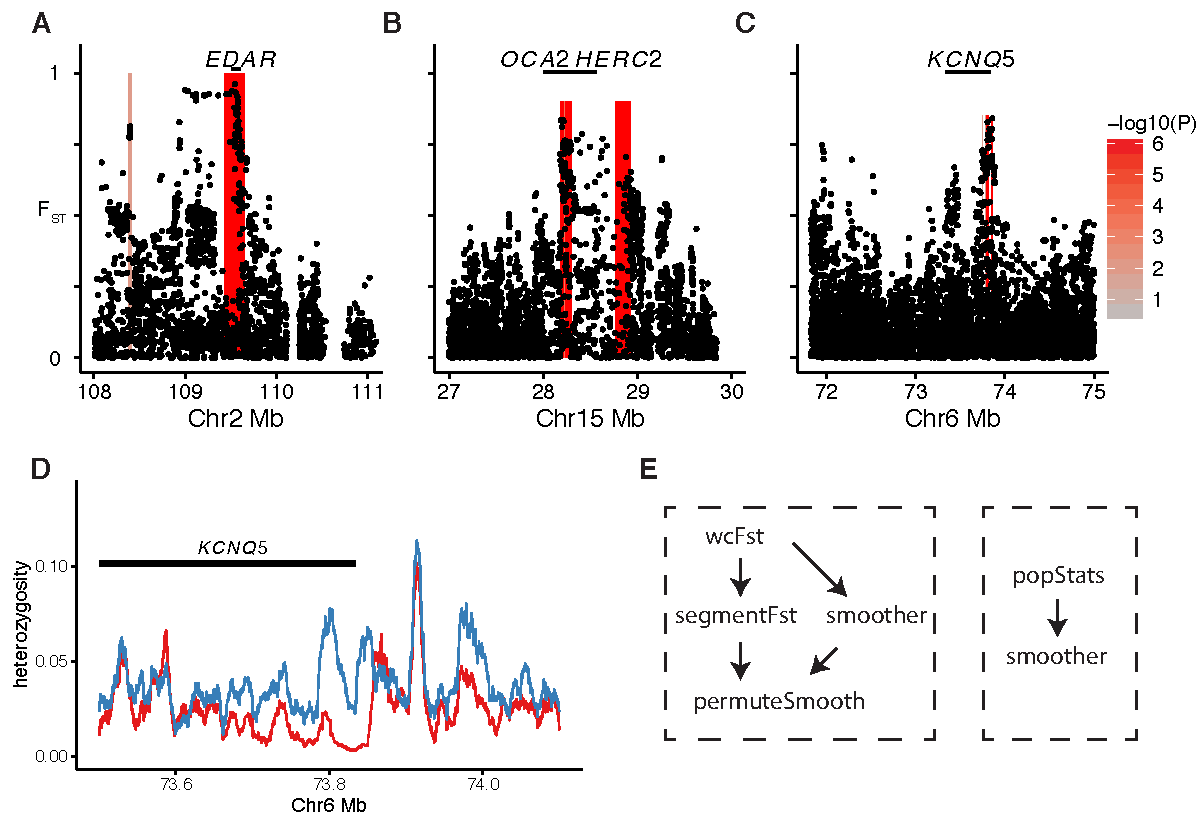
\includegraphics[width=0.95\textwidth]{Fig1}
\caption{{\bf Using VCFLIB to find population stratified loci in the One Thousand Genomes Project data.} The  F$_{ST}$  scatter plots (A-C) show genomic position on the x-axis and Weir and Cockerham's  F$_{ST}$  on the y-axis.  The vertical bands delineate regions of high  F$_{ST}$  defined by segment F$_{ST}$ .  The color of the bands denotes the empirical significance of the region compared to the rest of the genome determined with permuteSmooth.  A: EDAR is outlier in the CEU-CHB comparison because EDAR is under selection in CHB.  B: OCA2 and HERC2 are outliers in the CEU-CHB comparison because they are under selection in CEU.  The segmentation of the region is broken by segmental duplications between ~28-29 Mb.  C: KCNQ5 is an outlier in the CEU-YRI comparison.  D:  KCNQ5 shows decreased heterozygosity at it's 3' (~73.9Mb) end in CEU (red) compared with YRI (blue).  E: The GPAT workflows used for the  F$_{ST}$  analyses. }
\label{fig1}
\end{figure}

The three population pair-wise F$_{ST}$ comparisons resulting in over 30 million data points. To identify genomic regions with exceptional  F$_{ST}$  values we applied ``segmentFst" with a threshold of 0.6.   There were 3,790, 1,826, and 665 regions with high  F$_{ST}$  values for the CHB-YRI, CEU-YRI and CEU-CHB comparisons.  These regions overlapped 254 genes in CEU-CHB, 578 genes in CEU-YRI, and 1,047 genes in CHB-YRI.   To assess the empirical significance of the high  F$_{ST}$ regions we ran a permutation test for one million iterations.  At the most stringent cutoff (p $<$ 1e-5) there were 175 genes in CEU-CHB, 213 genes in CEU-YRI, and 407 genes in the CHB-YRI datasets.   

Classic examples of positive selection were present amongst our top hits. When comparing CHB to CEU, Ectodysplasin A receptor (\textit{EDAR}) was in a segment with the lowest p-value (1e-6) shown in Fig 1A. In a mouse model a single amino substitution in \textit{EDAR} affects hair thickness, the number of eccrine sweat glands and increased mammary glad branching \cite{edar}. We found CEU to be highly stratified around OCA2 and HERC, shown in Fig1B.  Variants in the OCA2 promoter, within a HERC2 intron, affect the expression of OCA2, a major loci for eye color\cite{oca2}.  

To test if there were  pathway enrichment for the stratified loci we ran DAVID with the highest classification stringency and constrained the analysis to segmented loci with and empirical p-value less than 1e-5. In all three gene lists there were no terms within functional clusters that reached significance after Benjamini-Hochberg correction.  While pathway enrichment was not fruitful, we noticed that there were a number genes expressed in the brain.  For example, \textit{KCNQ5} was highly differentiated between CEU and YRI, shown in Fig 1C.  Lowered heterozygosity in CEU was observed (Fig. 1D).  Dominant-negative \textit{KCNQ5} alleles, in mice, affect the after afterhyperpolarization of neurons in the CA3 hypocampus\cite{kcnq5}.  In another example, POGZ a gene that is has been associated with ID and autism spectrum disorders was found in the CEU-CHB comparison, see Fig S2.  While the patterns of F$_{ST}$ around many of these loci are consistent with selection, much more work is required to prove a significant correlation.

\subsection*{detecting within population selection using VCFLIB}


Segmentation of iHS data resulted in 1500, 1600, and 1937 regions in CHB, CEU, and YRI (segmentation threshold :  3).  For all three analyses a total of 1,885 unique genes were discovered.  In the CEU population lactase (\textit{LCT}) was amounts the highest scored regions shown in Fig. 2B.  The haplotype diversity around \textit{LCT} is noticeably different (Fig. 2C-D). CCR1,CCR3, RBFOX2,  YRI. 


\begin{figure}[h]

%\includegraphics[width=0.95\textwidth]{Fig2}
\caption{{\bf Using VCFLIB to identify patterns of haplotype diversity consistent with natural selection.} A: The GPAT 
workflows used for the haplotype analysis. B: Genome-wide iHS Manhattan plot for Norther Europeans (CEU).  The x-axis is an index and the y-axis is the average absolute iHS within a 100Kbs sliding window.  The repeating color palette delineates chromosomes.  Several iHS peaks are annotated with the closes gene or a dash if there was not a gene nearby. The window that overlaps lactase has the highest genome-wide average iHS.  C: The lactase haplotypes present in CEU and YRI.  Each row is a single haplotype and each column is a position where there is a non-reference allele (red).  Fewer unique haplotypes can be seen in CEU compared to YRI.   The trapezoid denotes where the haplotppe plots are in relation to lactase. D:  The Extended Haplotype Homozygosity (EHH) decay for rs3754686(A/G).  The position is shown on the x-axis and EHH for the derived (orange) and ancestral allele (green) is shown on the y-axis. 

}
\label{fig2}
\end{figure}



\section*{Availability and Future Directions}

VCFLIB is publicly available at (\url{https://github.com/ekg/vcflib}{VCFLIB}) and additional documentation can be found at \url{https://github.com/zeeev/vcflib/wiki}.  

Areas of continued development include extending documentation, unit testing,  support for new VCF specifications, and additional population genetic metrics.



\section*{Supporting Information}

% Include only the SI item label in the subsection heading. Use the \nameref{label} command to cite SI items in the text.
\subsection*{S1 Snakemake}
\label{S1_snakemake}
{\bf  F$_{ST}$  analyses.}  The snakemake file for the CEU-CHB  F$_{ST}$  analysis.  

\subsection*{S2 Snakemake}
\label{S2_snakemake}
{\bf iHS analyses.}  An archive of the snakemake file, the config file and region file used to run the CEU iHS analyses.

\subsection*{S1 Fig}
\label{S1_Fig}
{\bf Comparison of iHS methods.}  Scatter plots comparing VCFLIB's implementation of iHS to SELSCAN or Prichard's iHS. The iHS data are from a two megabase window around \textit{LCT} in CEU.

\subsection*{S1 Table}
\label{S1_Table}
{\bf Regions with high  F$_{ST}$  values.} The CEU-YRI, CEU-CHB, and CHB-YRI regions are in three different excel sheets.  The region in GRCh37 coordinates, the average  F$_{ST}$  values, and the empirical significance are listed as column headers.

\section*{Acknowledgments}

We would like to thank the countless number of people who have contributed suggestions, created bug reports, and modified the VCFLIB codebase.  

\subsection*{The VCFLIB Consortium}
\newline
\newline
EJ Osborne\textsuperscript{1},
Brett Kennedy\textsuperscript{1},
Daniel Ence\textsuperscript{1},
Travis Collier\textsuperscript{1},
EJ Osborne\textsuperscript{1},
...
\nolinenumbers

%\section*{References}
% Either type in your references using
% \begin{thebibliography}{}
% \bibitem{}
% Text
% \end{thebibliography}
%
% OR
%
% Compile your BiBTeX database using our plos2015.bst
% style file and paste the contents of your .bbl file
% here.
% 
\begin{thebibliography}{10}
\bibitem{1kg}
Sudmant, Peter H., et al. ``An integrated map of structural variation in 2,504 human genomes." Nature 526.7571 (2015): 75-81.

\bibitem{gonl}
Genome of the Netherlands Consortium. ``Whole-genome sequence variation, population structure and demographic history of the Dutch population." Nature Genetics 46.8 (2014): 818-825.

\bibitem{vcftools}
Danecek, Petr, et al. ``The variant call format and VCFtools." Bioinformatics 27.15 (2011): 2156-2158.

\bibitem{exac}
Exome Aggregation Consortium (ExAC), Cambridge, MA, http://exac.broadinstitute.org/, Feb 2016.

\bibitem{selscan}
Szpiech, Zachary A., and Ryan D. Hernandez. ``selscan: an efficient multithreaded program to perform EHH-based scans for positive selection." Molecular biology and evolution 31.10 (2014): 2824-2827.

\bibitem{voight}
Voight, Benjamin F., et al. ``A map of recent positive selection in the human genome." PLoS Biol 4.3 (2006): e72.

\bibitem{pigeon}
Shapiro, Michael D., et al. ``Genomic diversity and evolution of the head crest in the rock pigeon." Science 339.6123 (2013): 1063-1067.

\bibitem{tet}
Galati, Domenico F., et al. ``DisAp-dependent striated fiber elongation is required to organize ciliary arrays." The Journal of cell biology 207.6 (2014): 705-715.

\bibterm{b F$_{ST}$ }
Holsinger, Kent E., Paul O. Lewis, and Dipak K. Dey. ``A Bayesian approach to inferring population structure from dominant markers." Molecular Ecology 11.7 (2002): 1157-1164.

\bibitem{ F$_{ST}$ }
Weir, Bruce S., and C. Clark Cockerham. ``Estimating F-statistics for the analysis of population structure." evolution (1984): 1358-1370.

\bibitem{kim}
Kim, Su Yeon, et al. ``Design of association studies with pooled or un?pooled next?generation sequencing data." Genetic epidemiology 34.5 (2010): 479-491.

\bibitem{heng}
Li, Heng. ``A statistical framework for SNP calling, mutation discovery, association mapping and population genetical parameter estimation from sequencing data." Bioinformatics 27.21 (2011): 2987-2993.

\bibitem{color}
Domyan, Eric T., et al. "Epistatic and combinatorial effects of pigmentary gene mutations in the domestic pigeon." Current Biology 24.4 (2014): 459-464.

\bibitem{iron}
Barber, Matthew F., and Nels C. Elde. "Escape from bacterial iron piracy through rapid evolution of transferrin." Science 346.6215 (2014): 1362-1366.

\bibitem{tabix}
Li, Heng. ``Tabix: fast retrieval of sequence features from generic TAB-delimited files." Bioinformatics 27.5 (2011): 718-719.

\bibitem{edar}
Kamberov, Yana G., et al. ``Modeling recent human evolution in mice by expression of a selected EDAR variant." Cell 152.4 (2013): 691-702.

\bibitem{oca2}
Eiberg, Hans, et al. ``Blue eye color in humans may be caused by a perfectly associated founder mutation in a regulatory element located within the HERC2 gene inhibiting OCA2 expression." Human genetics 123.2 (2008): 177-187.


\bibitem{knq5}
Tzingounis, Anastassios V., et al. ``The KCNQ5 potassium channel mediates a component of the afterhyperpolarization current in mouse hippocampus." Proceedings of the National Academy of Sciences 107.22 (2010): 10232-10237.

\end{thebibliography}



\end{document}

